% !TEX TS-program = xelatex

\documentclass[10.5pt]{article}
\usepackage{fontspec}
\usepackage{polyglossia}
\usepackage{amsmath, amssymb}
\usepackage{multicol}
\usepackage{graphicx}
\usepackage{geometry}
\usepackage[table]{xcolor}
\usepackage{array}
\usepackage{wrapfig}
\usepackage{caption}
\usepackage{setspace}


\setdefaultlanguage{russian}
\setmainfont{Liberation Serif}

\geometry{a4paper, top=1.2cm, bottom=1.6cm, left=1.6cm, right=1.8cm, nofoot}


\setstretch{1.15}
\setlength{\columnsep}{0.5cm}

\newcommand{\ang}[1]{\angle{#1}}

\pagestyle{empty}

\begin{document}

% Подключаем титульный лист
% !TEX TS-program = xelatex

\thispagestyle{empty}

\begin{center}
    \vspace*{2cm}
    {\LARGE\textbf{ЖУРНАЛ «КВАНТ»}}\\[1.5cm]
    
    {\Large\textbf{МАТЕМАТИКА $\cdot$ ФИЗИКА}}\\[2cm]
    
    {\LARGE\textbf{ОТВЕТЫ, УКАЗАНИЯ, РЕШЕНИЯ}}\\[0.5cm]
    {\large\textbf{(к задачам из выпусков №5--6)}}\\[3cm]
    
    {\large\textbf{№ 6 $\cdot$ 1998}}\\[14cm]
    
    {\large\textbf{МОСКВА $\cdot$ 1998}}
\end{center}

\clearpage

% Подключаем статью
% !TEX TS-program = xelatex

\begin{center}
    \Large{ОТВЕТЫ, УКАЗАНИЯ, РЕШЕНИЯ}
\end{center}
\vspace{-0.2cm}
\hrule height 0.6pt
\vspace{-0.2cm}


\begin{multicols}{2}

% ===== ЛЕВАЯ КОЛОНКА =====
\noindent
«КВАНТ» ДЛЯ МЛАДШИХ ШКОЛЬНИКОВ
\vspace{0.3cm}

\noindent
ЗАДАЧИ \\
\small
\vspace{0.1cm}
\textit{(см. «Квант» №5)}

\vspace{0.1cm}
\noindent
\textbf{1.} Заднее колесо трактора за секунду совершит ровно один оборот.

\noindent
\textbf{2.} См. таблицу:


\setstretch{1.3}

\begin{center}
\setlength{\tabcolsep}{3pt}
\renewcommand{\arraystretch}{1.2}
\begin{tabular}{|c|c|c|c|c|c|}
\hline
 & \textbf{7«А»} & \textbf{7«Б»} & \textbf{7«В»} & \textbf{7«Г»} & \textbf{$\Sigma$} \\
\hline
\textbf{7«А»} & \cellcolor{gray!80} & 3:0 & 2:1 & 2:0 & 7:1 \\
\hline
\textbf{7«Б»} & 0:3 & \cellcolor{gray!80} & 0:0 & 2:0 & 2:3 \\
\hline
\textbf{7«В»} & 1:2 & 0:0 & \cellcolor{gray!80} & 2:1 & 3:3 \\
\hline
\textbf{7«Г»} & 0:2 & 0:2 & 1:2 & \cellcolor{gray!80} & 1:6 \\
\hline
\end{tabular}
\end{center}

\setstretch{1.05}

\noindent
\textbf{3.} Обозначим угол $AOB$ через $\alpha$, тогда $\ang{AOD} = \dfrac{\alpha}{2}$, а \\

\noindent
$\ang{DOC} = \dfrac{\pi}{2} - \dfrac{\alpha}{2}$. Угол $COB$ равен $\alpha - \dfrac{\pi}{2}$, а $\ang{COE} = \dfrac{\alpha}{2} -$\\

\noindent
$-\dfrac{\pi}{4}$. Следовательно, $\ang{DOE} = \ang{DOC} + \ang{COE} = \left(\dfrac{\pi}{2} - \dfrac{\alpha}{2}\right)$\\

\noindent
$+ \left(\dfrac{\alpha}{2} - \dfrac{\pi}{4}\right) = \dfrac{\pi}{4}$.

\vspace{0.3cm}
\noindent
\textbf{4.} Разобьем гирьки на 50 пар соседних гирек. Затем эти 50 пар разобьем на две кучки по 25 пар. Теперь из первой куч-\\
ки положим на левую чашку весов тяжелую гирьку из каждой пары, а на правую~--- более легкую. Со второй кучкой поступим наоборот~--- на левую чашку положим более легкие гирьки из пар, а на правую~--- более тяжелые. Очевидно, что в результате весы окажутся в равновесии.

\noindent
\textbf{5.} Судья не всегда может сделать расписание на оставшиеся 2 дня. Например, если в первые три дня команды играли

\begin{minipage}{0.9\linewidth}
    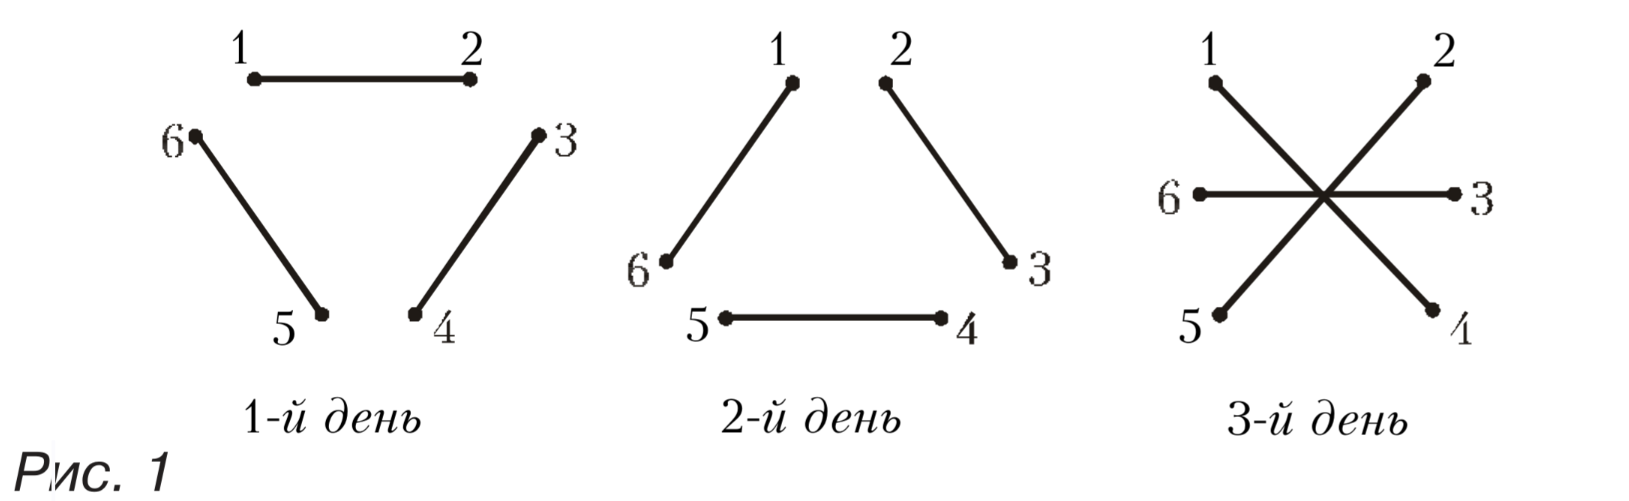
\includegraphics[width=\linewidth]{pic1.png}
\end{minipage}


\noindent
так, как показано на рисунке~1 (отрезками соединены номера команд, играющих в этот день), невозможно было бы устроить расписание даже только на четвертый день. Действительно, команда с нечетным номером может играть лишь с командами, имеющими нечетные номера, но таких команд три, следовательно, одной из них не с кем будет играть в четвертый

\vspace{0.3cm}

\noindent
\textit{(см. «Квант» №6)}

\vspace{0.1cm}
\noindent
\textbf{1.} Смогут. Поскольку Буратино не хватает 18 сольдо, а Мальвине не хватает 7 сольдо, у Мальвины есть по крайней мере $18 - 7 = 11$ сольдо. Если она добавит их к деньгам


\begin{wrapfigure}{l}{0.62\columnwidth}
    \vspace{-0.4cm}
        \centering
        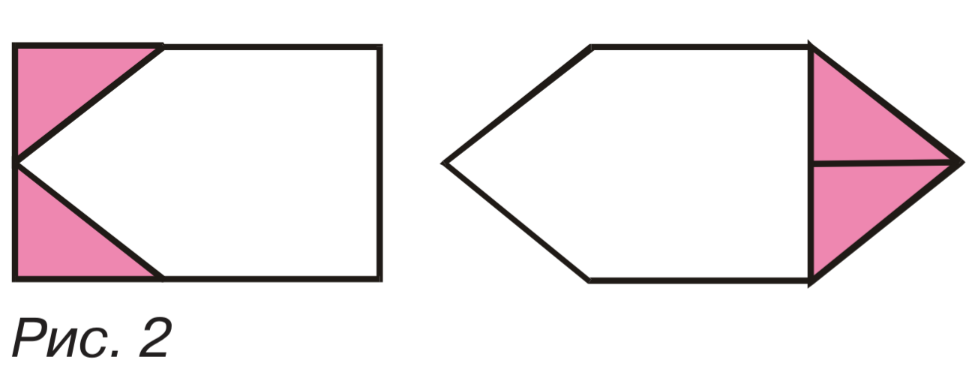
\includegraphics[width=\linewidth, height=75pt]{pic2.png}
        \centering
        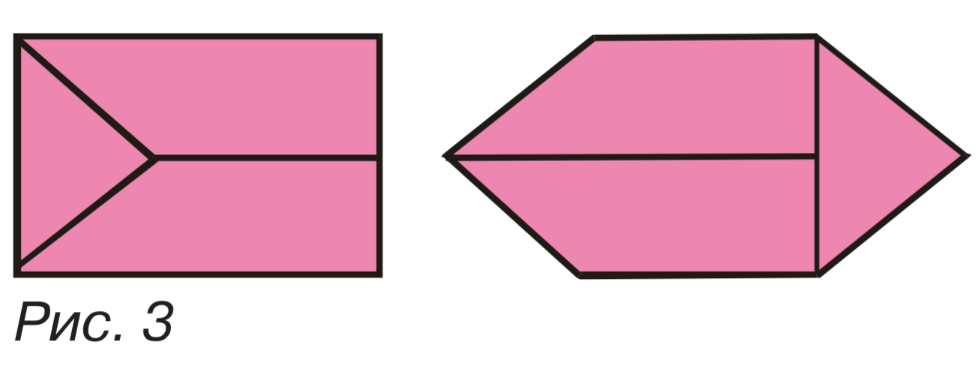
\includegraphics[width=\linewidth, height=75pt]{pic3.png}
    \vspace{-1cm}
\end{wrapfigure}

\noindent
Пьеро, то денег на букварь, конечно же, хватит.

\noindent
\textbf{2.} См. рис. 2, 3.

\noindent
\textbf{3.} Число 220 нельзя представить в виде суммы двух натуральных чисел, все цифры которых нечетны.


\noindent
\textbf{4.} 1665. Сумма последних цифр трех исход-

\columnbreak


% ===== ПРАВАЯ КОЛОНКА =====
\noindent
ных трехзначных чисел оканчивается на 5. Числа 5 и 25 не представимы в виде суммы трех ненулевых различных цифр. Значит, сумма последних цифр равна 15. Тогда сумма средних цифр тоже равна 15, и сумма первых цифр тоже 15. Те-\\

\begin{wrapfigure}{r}{0.52\columnwidth}
    \vspace{-0.3cm}
    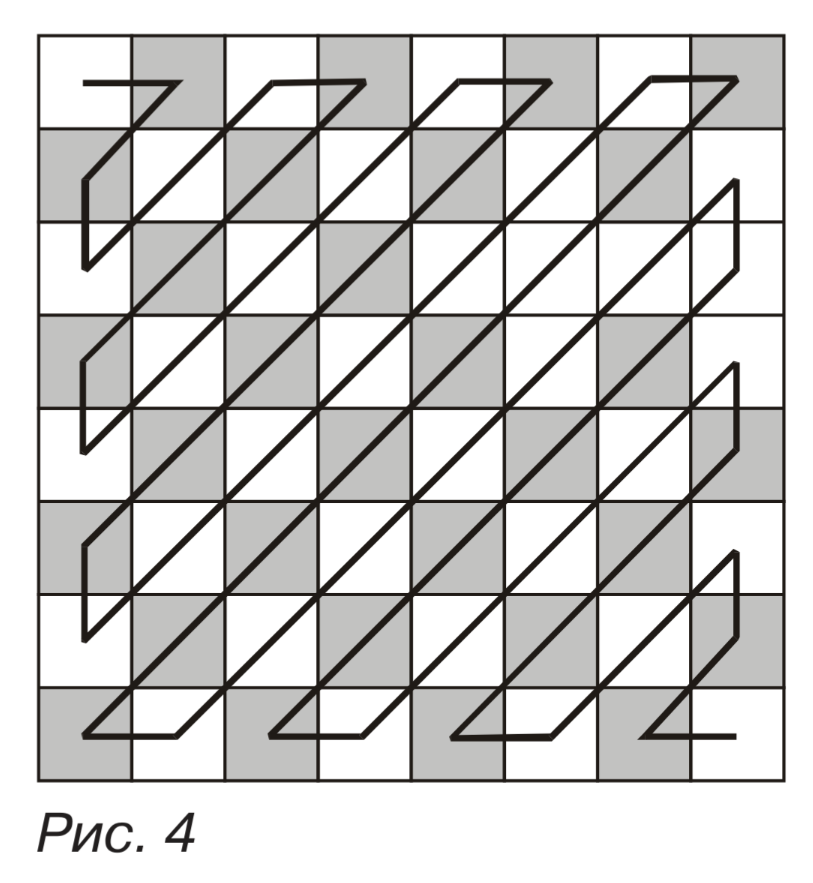
\includegraphics[width=\linewidth]{pic4.png}
    \vspace{-1cm}
\end{wrapfigure}

\vspace{-0.4cm}
\noindent
перь ясно, что после перестановки мы получим три числа, сумма которых 1665.

\noindent
Напоследок предъявим тройку чисел (одну из возможных), которая удовлетворяет условию задачи: 159, 672, 834.

\vspace{0.2cm}
\noindent
\textbf{5.} На рисунке 4 король сделал 49 диагональных ходов. Доказать, что число 49 максимально возможное, очень просто. Каждый диагональный ход проходит через один узел шахматной доски. (Узлом мы здесь называем общую точку 4 клеток шахматной доски.) Всего узлов 49. Два раза пройти через один и тот же узел без самопересечения пути невозможно.

\vspace{0.3cm}
\noindent
\large
МЕТАМОРФОЗЫ ПОСЛЕДОВАТЕЛЬНОСТЕЙ

\vspace{0.1cm}
\small
\noindent
\textbf{1.} П$_9$, П$_{10}$, П$_{11}$. Если считать, что в момент отплытия лодки отправляется автобус №0, то турист должен сесть в автобус №66. (Решение аналогичной задачи см. на с. 87--88 в журнале «Квант» №1/2 за 1993 г.)

\vspace{0.2cm}
\noindent
\textbf{2.} 
$P_4(x) = x^4 + 2x^3 + x^2 - \dfrac{1}{30}$,\\
$S_4(n) = \dfrac{1}{5}n^5 + \dfrac{1}{2}n^4 + \dfrac{1}{3}n^3 - \dfrac{1}{30}n = \dfrac{n(n+1)(2n+1)(3n^2+3n-1)}{30}$.

\vspace{0.2cm}
\noindent
\textbf{3.} $S_k(0) = \int\limits_0^0 P_k(x)\,dx = 0$.

\vspace{0.2cm}
\noindent
\textbf{4.} \textit{Указание.} Коэффициент при старшей степени многочлена $P_k(x)$ равен 1.

\vspace{0.2cm}
\noindent
\textbf{5.} $-\dfrac{1}{2} + \dfrac{(-1)^n}{2\cos\dfrac{1}{2}}\cos\left(n + \dfrac{1}{2}\right)$.

\vspace{0.2cm}
\noindent
\textit{Указание.}
\[
\sum_{k=1}^n (-1)^k \cos k = \dfrac{1}{2}\sum_{k=1}^n \left(\cos(\pi+1)k + \cos(\pi-1)k\right).
\]

\vspace{0.2cm}

\noindent
\large
АНАЛОГИИ В ЗАДАЧАХ ПО ФИЗИКЕ
\vspace{0.2cm}

\small
\noindent
\textbf{1.} $T = \dfrac{kq\lambda}{R}$. \quad
\textbf{2.} $T = \sigma R$. \quad
\textbf{3, 4, 5.} $\Delta W = -W_0/2$.

\vspace{0.2cm}
\noindent
\large
МОСКОВСКИЙ ФИЗИКО-ТЕХНИЧЕСКИЙ ИНСТИТУТ
\vspace{0.2cm}

\small
\noindent
МАТЕМАТИКА

\vspace{0.2cm}
\noindent
\textit{Вариант 1}

\noindent
\textbf{1.} $x = \pm \dfrac{3\pi}{4} + 2\pi k, \ k \in \mathbb{Z}$. \textit{Указание.} В каждом из случаев $\cos x > 0$ и $\cos x < 0$ выполните подстановку $t = \dfrac{\cos 3x}{\cos x}$.

\vspace{0.2cm}
\noindent
\textbf{2.} $x < \dfrac{34 - 30\sqrt{2}}{23}$, \ $x \geq 3$.

\vspace{0.2cm}
\noindent
\textbf{3.} $\dfrac{5\sqrt{34}}{12}$. \textit{Решение.} Точка $D$ является центром описанной около треугольника $ABC$ окружности, $AB = 5$, $AC = 4$. Пусть $O_1$~--- центр окружности, вписанной в равнобедренный

\end{multicols}

\end{document}

\end{document}